\chapter{Heretic Purging}

\begin{wrapfigure}{O}{\figwidth}
	\begin{center}
		
\includegraphics[width=\figwidth]{pics/6/1.png}
	\end{center}
\end{wrapfigure}
This is the ongoing tale of a bunch of guardsmen who got drafted into the Inquisition after their regiment was reduced to a mere 37 men by a combination of Orks, Heretics, more Orks, Tyranids and, of course, their own leadership. 
Currently they work for an Inquisitor that is the 40k equivalent of Professor Oak, he provides teams and missions to Interrogators who need to get some leadership experience before becoming full Inquisitors. 
The lot of these guardsmen is rather thankless, they are matched up with five other less combat focused team members, assigned to an Interrogator, and sent out to fight the enemies of the Imperium.

%>Most previous chapters can be found here:
%http://suptg.thisisnotatrueending.com/archive.html?searchall=all+guardsmen

The squad has just boarded the shuttle to their next mission behind the familiar forms of the Interrogator better known as 'the Rupert', and his manservant Alfred. 
As they enter the shuttle's conference room the Interrogator introduces the guardsmen to the rest of the team and begins regaling everyone with the story of his previous mission with the squad. 
An elderly woman, a small weasley man, a cleric, and a tall man in a duster are listening to the Rupert's tale with a mixture of confusion and disbelief.

Sarge is listening to the Rupert and occasionally wincing and muttering corrections when enthusiasm gets the better of memory. 
Twitch has backed himself into a corner and is glaring at his new teammates while he fiddles with a proximity mine. 
Doc is helping Alfred serve tea and trying to keep Cutter out of the way as the melee specialist wolfs down snacks. 
The squad's new member, the flame trooper Crisp, is laughing heartily at the Interrogator's story while thumping an uncomfortable looking cleric on the back. 
As they do all this the squad vaguely wonders what the Rupert had meant by 'theological trouble'.

\begin{wrapfigure}{O}{\figwidth}
	\begin{center}
		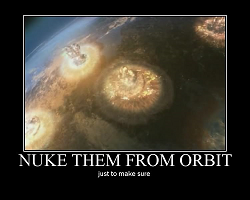
\includegraphics[width=\figwidth]{pics/6/2.png}
	\end{center}
\end{wrapfigure}
So no shit there we were, on our way to a planet that had separated from the Imperium for a few centuries to ask the locals why they had turned away from light of the God Emperor. 
This was not something we were even remotely qualified for, so we were a all a little confused about why we had been sent. 
Technically rooting out Heresy is what the Inquisition is all about, but this was an entire planet that had forgotten the Imperial Creed, not some cult of daemon worshipers hiding in the sewers. 
We all knew this was the sort of shit the Ecclesiarchy was made for, none of us were happy with the idea that we might be edging in on their turf.

After the Rupert finished his little story and had his tea, Sarge decided it was time to find out just what sort of shitstorm we were heading into. 
In his typical rambling fashion our Interrogator told us the tale of Ork invasions, Imperial retreats, scorched earth tactics, and plucky survivors. 
We dismissed most of it as bullshit, but the core of the matter seemed to be that a few hundred years ago a major Waaagh had cut through the sector forcing a general retreat. 
As part of this retreat the Imperium had strategically abandoned a planet and nuked it on the way out to keep the Orks off it. 
Now that we were finally pushing back the Orks and the radiation was fading, that planet was going to be integrated back into the Imperium. 
The first step of this process involved inducting as many of the survivors as possible into the Guard. 
These people were practically deathworlders after all and the Guard can always use more deathworlders.

The only problem was that these yokels didn't Praise the Emperor and you can't have men like that in the Guard. 
So the Ecclesiarchy was called in and was doing its best to spread the faith and stamp out the more heretical local religions. 
Something they ran into spooked them though, so now we were coming in to see just how heretical these people were.

\begin{wrapfigure}{O}{\figwidth}
	\begin{center}
		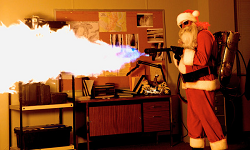
\includegraphics[width=\figwidth]{pics/6/3.png}
	\end{center}
\end{wrapfigure}
To no ones surprise our Interrogator was an old family friend of our ship's captain, so instead of being treated as an uppity form of cargo we were welcomed as honored guests and given real quarters. 
It was nice travelling with with the Rupert, a guardsman can sleep anywhere but there's something to be said for a bed with actual sheets. 
We settled into our quarters, got the perimeter defenses up, and got to know the rest of the team.

Nubby's replacement in the squad was Crisp, a big jolly flamer expert who the rest of us found vaguely unsettling. 
Just to be clear, we all liked Crisp; he had been the best damned cook in the regiment, was always laughing and joking, and could put a stream of burning promethium through the firing slits of an oncoming tank like it was nothing. 
He hadn't taken the regiment's death well though, he had been everyone's friend and all the deaths hit him hard. 

He started losing weight and stopped laughing after he joined the Inquisition and from what we heard his squad's missions had been especially horrific. 
Every time we saw him between deployments he had looked worse and worse. 
None of us had expected him to last much longer, but something had changed on his last mission. 
He was eating and joking again and loved trading stories with the Rupert, it was just that his jokes didn't always make sense and his smile was a bit too wide. 
We'd all seen guardsmen bend under pressure, and both Twitch and Cutter had practically snapped, but Crisp's fixed smile and slightly twisted humor worried the rest of us.

\begin{wrapfigure}{O}{\figwidth}
	\begin{center}
		
\includegraphics[width=\figwidth]{pics/6/4.png}
	\end{center}
\end{wrapfigure}
The rest of the team was less disturbing than Crisp. 
The Rupert and Alfred were the same as we remembered then, except for the masterwork augmetic that had replaced the Rupert's charred stump of an arm. 
Our Interrogator had handpicked several experts for this mission in addition to us guardsmen. 
For working with the locals there was an Arbite who had experience keeping the peace on feral and frontier worlds as well as a greasy man who had served as a translator and negotiator on a Rogue Trader. 
The religious investigation would be aided by a cleric who had worked as a missionary for several years and a tiny old woman of an adept who knew just about everything; 
we liked her, she didn't take shit off anybody and delighted in making Doc and Alfred uncomfortable.

We didn't even bother trying to keep ourselves walled off from the rest of the team, after our last mission with the Rupert we knew that he wouldn't let us get away with it. 
We suffered through lectures on the Imperial creed and acceptable deviations from the cleric and adept, basic language lessons from the greaseball and adept, and lessons on frontier law from the arbite and, of course, the adept. 
It was like being back in school, right down to the little old lady hitting us when we didn't pay attention.

The whole experience was rather degrading, aside from Doc none of us were cut out for higher learning, we were guardsmen not bloody diplomats. 
We couldn't duck out of it though, so we spent our trip like a bunch of officer cadets; 
busting our asses in PT and being force-fed trivia by frustrated teachers all day, listening to the ramblings of an old warhorse in the evening, and sleeping like the dead all night. 
The trip slowly continued and we suffered, but at least we knew that we'd be ready for anything the mission threw at us, compared to this torture purging a bunch of heretics would be a walk in the park.

\begin{wrapfigure}{O}{\figwidth}
	\begin{center}
		
\includegraphics[width=\figwidth]{pics/6/5.png}
	\end{center}
\end{wrapfigure}
We made planetfall at the fortified camp that the surveyors were using as their main shuttleport. 
The place was within spitting distance of one of the irradiated cities and it was disconcerting to see the towers standing completely motionless and silent in the distance. 
The various leaders of the expedition came out to greet us and for a change everyone seemed happy to see Inquisition, it was weird. 

We spent the next few days wining and dining with Munitorum, Ecclesiarchy, Administratum, and Mechanicus officials of varying degrees of unpleasantness. 
We managed not to thoroughly embarrass ourselves, but for some reason none of the survey's leaders was willing to tell us the exact reason that we had been summoned.
We got a lot of vague and contradictory information, but everyone seemed to have a political agenda here and wanted to make sure we'd act in their interest before they told us anything useful. 
We couldn't even find the Pontifex who had asked for our help, apparently he'd gone off to negotiate with some local priests and hadn't come back yet. 
We didn't have time for this shit so we decided to stop pussyfooting around and find someone who didn't have their head stuck up their ass.

While the Rupert and Alfred kept the obnoxious big wigs busy while we split into pairs found the various assistants and secretaries that did the actual work, then shook them down for information. 
Doc and the Adept talked to the Mechanicus while the Arbite and the Greaseball asked the Administratum some questions. 
The cogboys and pencil pushers didn't have anything useful for us; just a lot of junk about radiation levels, incoming colonists, recovering biospheres, and irradiated manufactorums. 
The rest of the team had better luck getting useful intel, except for Twitch who was left in base because he was still banned from investigating anything ever again.

\begin{wrapfigure}{O}{\figwidth}
	\begin{center}
		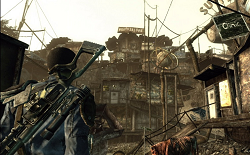
\includegraphics[width=\figwidth]{pics/6/6.png}
	\end{center}
\end{wrapfigure}
Sarge and Cutter managed to find a very helpful lad working in the Munitorum who knew all about the locals. 
Apparently they were the hardest bastards this side of catachan, had a very clear memory of who nuked them into the stone-age, and had been spending the last few hundred years rebuilding their civilization and fighting with the remnants of the Orkish invasion. 
They had built several small cities, mostly over the underground bunkers that had sheltered their forefathers, which they defended with a mixture of primitive weaponry and scavenged Imperial tech. 
The locals weren't overtly hostile towards the Imperium, since most of them saw re-assimilation as a great improvement over their current living conditions, but they had abandoned the Imperial faith and developed about fifty different religions of their own.

Crisp in the Cleric, who were paired up for obvious reasons, had to search the entire Ecclesiarchy camp before they found someone useful, a Sister Dialogous who had been keeping track of everything. 
According to her the Ecclesiarchy had been spreading the Imperial Creed with a fair degree of success before shit went south. 
In a single night nearly all of the active missionaries had been attacked by assassins or angry mobs, but Ministorum missionaries are tough bastards and several of them killed their attackers and made their escape. 
In response to these attacks a few squads of Sisters of Battle were deployed to sort things out, a little examination of the deceased assassins led them to one of the smaller religions near an irradiated city. 
The sisters went in, some serious shit went down, and about half the sisters came back out. 
They declared the place purged then put it under quarantine and called for us.

None of this was exactly good news, but at least we knew the gist of what was going on and where to go next. 
A flier was requisitioned and we all headed out to talk to the sisters.

\begin{wrapfigure}{O}{\figwidth}
	\begin{center}
		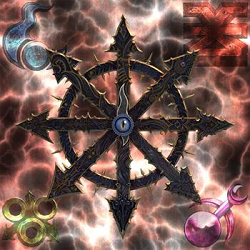
\includegraphics[width=\figwidth]{pics/6/7.png}
	\end{center}
\end{wrapfigure}
We geared up for a fight as we flew, whatever the sisters had run into had chewed them up pretty badly and we weren't going to take their word it was dead. 
We landed right at the edge of one of the nuked cities, we were close enough that all of us had to wear rebreathers and Doc warned us not to stay too long if we ever wanted to have children. 
The sisters had set up a perimeter around a large ruined building and set up a field barracks, as we approached a senior sister came out and the Rupert flashed his rosette.

The sister superior took us towards the ruined building and filled us in as we walked. 
She had been sent here with three squads to purge the temple, they had rolled over the guards and busted down the door in seconds.
They had expected to find cultists and fanatics inside, they hadn't expected a horde of mutants backed up by psykers. 
You gotta give the sisters credit for sheer bloody perseverance, they stood their ground and killed them all, taking fifty percent casualties in the process but completing the objective. 
Poor, dumb, zealots, that sort of shit is what the Emperor gave us indirect fire support for.

The reason we were called was apparent the second we entered the building. 
Sitting on the wall behind the altar, glowing like a big glowy thing, was a Mark of Tzeentch. 
Underneath it were the much smaller marks of Nurgle, Khorne, and Slaanesh and above it was the symbol of Chaos Undivided. 
Sarge started swearing under his breath.

\begin{wrapfigure}{O}{\figwidth}
	\begin{center}
		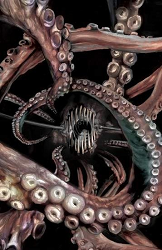
\includegraphics[width=\figwidth]{pics/6/8.png}
	\end{center}
\end{wrapfigure}
Our training had been fairly clear on what to do in this sort of situation, we asked the Adept and the Cleric to take a look while the rest of us averted our eyes. 
When they were done Crisp moved forward and drenched the whole thing in burning promethium while Twitch prepped a det-pack. 
The sister superior hit Crisp in the side with a flying tackle a second before a tentacle whipped out of the burning mark and speared the spot where he'd been standing. 
As we watched a dozen more tentacles squirmed out and the sister screamed at us to run or fight. 
We chose both.

We all backpedaled madly while pouring a steady stream of lasfire into the writhing mass, but the tentacles were emerging faster than we could shoot them. 
The Interrogator's and the Sister's bolters were having the best effect so it was no surprise that several of the larger tentacles slashed out at them. 
The Rupert drew his sword and parried the ones aimed at him, but the sister was knocked to the ground and a clawed tentacle seized her by the leg. 
Cutter saw his chance and started hacking at the limb dragging her away while Crisp seized her by the arms and pulled her to safety.

The tentacles were all focused on Cutter and the Rupert now, who were both carving off any limb that came near them. 
They were actually starting to push forward and it was a fair bet they could take the thing on and win, but we didn't feel like taking the risk so we all popped frags. 
The grenade barrage severed the tentacles at the base and gave both Cutter and the Rupert time to fall back to the rest of us. 
We all slowly backed to the doorway as the tentacles regrew and vainly tried to reach us. 
When we all had exited the mass withdrew into the mark which resumed glowing.

\begin{wrapfigure}{O}{\figwidth}
	\begin{center}
		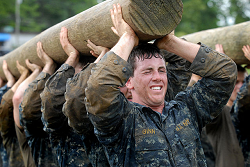
\includegraphics[width=\figwidth]{pics/6/9.png}
	\end{center}
\end{wrapfigure}
None of us had any desire to go back into the temple, but the chaos marks couldn't really be left there. 
The Rupert told Sarge to take the squad and figure out a way to get rid of them while the rest of the team took the wounded sister superior to her barracks. 
As they walked into the large tent that undoubtedly contained several hot chicks changing out of their hot, sweaty armor, we stood around and argued about how to deal with a tentacle daemon. 
There's no bloody justice.

Several of us were in favor of calling in an orbital strike, what's the point of being in the Inquisition if you can't go completely overkill? 
Sarge disagreed though, so we all took a walk around to the back side of the temple. 
Sarge proposed that we slap detpacks onto the back of the wall with the marks, but Twitch raised concerns about getting speared through the brickwork while the charges we planted. 
These were valid points, so while Twitch prepped several detpacks with adhesive Sarge had the rest of us root around in the rubble for any pipes or beams we could get our hands on, then we taped them together. 

Imagine, if you will, a forty foot pole made of taped together scrap metal. 
Now imagine there's a detpack stuck to one end of it and five sweating guardsmen holding up the other end, who knows what the sisters watching the perimeter thought of us. 
It worked though, mostly. 
We stuck five detpacks to the back wall of the temple, right behind where the mark was, and only dropped two of them on the ground. 
We all fell back to a safe distance, took cover and hit the detonator.

When we peeked out of cover the wall was gone, along with the marks and half the temple. 
With our heads held high we headed to the barracks to inform the Interrogator, hoping against hope that there might still be some hot undressed chicks inside. 
Unfortunately there weren't any half-naked sisters in the barracks when we got there, but we did get to see Doc have a heart attack.

\begin{wrapfigure}{O}{\figwidth}
	\begin{center}
		
\includegraphics[width=\figwidth]{pics/6/10.png}
	\end{center}
\end{wrapfigure}
Well it wasn't really a heart attack, it was damned close though. 
The first thing we saw when we entered was the sister superior lying on a table as a sister hospitaller treated her bloody leg. 
The second Doc laid eyes on the Hospitaller he started hyperventilating and tried to hide behind Sarge, unfortunately guard-issue rebreathers aren't exactly quiet devices. 
All conversation in the tent was halted by what sounded like a metal grate being attacked with a pushbroom. 

Everyone, including the wounded sister superior, turned to face Doc who started to turn an alarming shade of crimson and claw at his mask. 
Crisp and the old Adept broke into gales laughter as the Hospitaller ran over to see what was wrong with Doc, only Sarge's assurance that everything was fine saved the poor boy from terminal embarrassment. 
The rest of us removed our masks then Sarge, grinning like a schoolboy, gave a report to the Rupert that was occasionally interrupted by inexplicable coughing fits, these usually happened when he looked at Doc. 

Matters were not helped by both the Adept and Crisp making dirty jokes about 'playing doctor' in the background.

\begin{wrapfigure}{O}{\figwidth}
	\begin{center}
		
\includegraphics[width=\figwidth]{pics/6/11.png}
	\end{center}
\end{wrapfigure}
Eventually Sarge finished explaining our solution to the daemon problem and introduced the rest of the team to the Hospitaller we had met on our first mission. When the novelty of teasing Doc had worn off and he'd regained his composure the embarrassed medic went over to help patch up the sister superior's leg. 
While he did this the rest of us argued about just what the hell was going on on this planet. 

We knew the planet was filled with mundane heresy and had expected to have to deal with some minor daemon cults, but this had been a full blown Tzeentchian temple right down to the arcane symbols, horrific mutants, and tentacle monsters. 
On top of that the other chaos symbols seemed to suggest that each of the gods had a cult on this world and they were all working together in some way. 
It was a wonder that the planet hadn't been sucked into the warp or something.

\begin{wrapfigure}{O}{\figwidth}
	\begin{center}
		
\includegraphics[width=\figwidth]{pics/6/12.png}
	\end{center}
\end{wrapfigure}
The elderly Adept suggested tracking the other cults down and purging them, our squad was in favor of sitting tight and calling for reinforcements, and the Cleric wanted to exterminatus the planet on general principle. 
Eventually the Rupert settled the matter in the Adept's favor causing the Cleric to storm out of the tent while the Adept cackled and made obscene gestures at his back. 
We weren't exactly in favor of this plan, but we had expected it; the Rupert wasn't the sort of man to back down from a challenge.

Of course finding the cults wouldn't be easy. 
These were heretics hiding from the Imperium, it's not like they advertised and gave out pamphlets. 
It would take tireless searching, careful examination of evidence, and brilliant deduction to find the hidden temples; it was a near impossible task. 
We had to try though, so we all went with the arbite to search the remains of the temple for clues while the rest of the team questioned the sisters.

Within five minutes Crisp found a pamphlet advertising the 'Pit of Carnal Pleasures and Daemonic Delights' sitting on a table in the temple.

\begin{wrapfigure}{O}{\figwidth}
	\begin{center}
		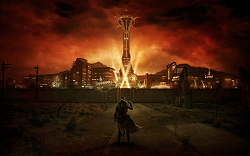
\includegraphics[width=\figwidth]{pics/6/13.png}
	\end{center}
\end{wrapfigure}
The pamphlet and its intriguing contents was handed over to the Adept and Cleric for inspection. 
They confirmed that this was almost certainly the Slaaneshi cult we were looking for, so we collected our gear and got ready to pay the place a visit. 
The sisters were also getting ready to leave as well, they'd shown us the marks and the temple was pretty much wrecked so the perimeter as no longer necessary. 
They were going to go assist the Pontifex in his negotiations with one of the local religious orders, but they gave us their contact code so we could vox them if we needed backup. 
The Adept congratulated Doc on getting the pretty girl's number.

The pamphlet pointed us towards a bunker underneath one of the larger towns that been built by the survivors. 
By the wastelanders' standards this was a rich settlement, it was a major local trade hub and had a fair sized standing army to keep things civil. 
There'd been some Imperial contact and trade with the local nobility, so we probably wouldn't be shot on sight, but we didn't think they'd be keen on us purging the bunker. 
The Rupert was all for marching in, declaring our authority, and having the local nobs aid us in our mission. 
The rest of us thought this sounded like a good way to get ourselves killed.

We argued the point with him and eventually came to a compromise; the Rupert and a few others would fly in and be diplomatic while the rest of the team would come in disguised and check out the possible cult. 
The plan called for the Rupert to make friends and slowly work the town's leaders up to the idea of helping us over a few days, if we ran into anything chaosy we'd call for him and he'd convince the locals to help us. 
None of the squad had any faith in his ability to convince the wastelanders to side with us, so we had absolutely no intention of calling him for anything short of a Bloodthirster.

\begin{wrapfigure}{O}{\figwidth}
	\begin{center}
		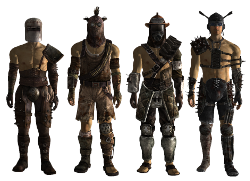
\includegraphics[width=\figwidth]{pics/6/14.png}
	\end{center}
\end{wrapfigure}
We stopped at a small tradepost and exchanged a few of our surplus weapons for sets of local clothing and armor. 
The Arbite and the Greaseball helped get us into disguise and prepped us on local slang and customs, then we split up a few hours walk outside town. 
The diplomatic team consisted of the Rupert and Alfred as well as the Greaseball and the Cleric, they had a full spectrum of diplomatic skills at their disposal and the two teammates who most annoyed us were out of our hair. 

As the rest of us started the long hike to the town behind the Arbite we speculated on what sort of trouble the diplomatic team would get into. 
Twitch thought they were all going to sacrificed to the dark gods, Crisp painted some rather scandalous scenarios involving the Greaseball that made us rather uncomfortable just hearing about, and the rest of us had our money on the Rupert challenging someone to a duel. 
The Adept had a few interesting theories of her own, but the Arbite ignored us and muttered to himself about 'standards' and 'professionalism'.

The Arbite talked us through the town's gates as mercenary escorts for the Adept, between our scrap armor and well used weaponry we certainly looked the part.
There was a bit of an argument over bringing Crisp's flamer inside the settlement, a quick bribe and a close look at Cutter's chainsword sorted that out though.
Once inside it was damned easy to find the 'Pit of Carnal Pleasures and Daemonic Delights', apparently it was the major attraction around here. 
Unfortunately it was a lot harder to get into than to find, several armed guards were stationed around the large vault door that served as the entrance to the bunker and they refused to let us in with our weapons.

\begin{wrapfigure}{O}{\figwidth}
	\begin{center}
		
\includegraphics[width=\figwidth]{pics/6/15.png}
	\end{center}
\end{wrapfigure}
We rented a room for the night and tried to figure out a way into the Pit without abandoning our weapons or bringing the entire settlement down on us. 
None of us were stealthy enough to sneak in, we couldn't find any alternate entrances, and the guards were notoriously unbribable; 
the only thing we could think of was trying to hide our weapons inside our clothing, but after our previous meeting with the guards they were sure to search us. 
We agonized over this for several hours before the Adept came to our rescue, she was sure she could carry handguns for each of us past the guards along with any small gadgets we needed.

The next evening we returned to the Pit, not as individual customers, but as escorts for the Adept. 
The guards did a double-take at this, their usual clientele probably didn't include tiny old women and nothing could have prepared them for how the Adept acted. 
We knew the Adept was feisty and we had all heard her tease Doc, but the things that came out of her mouth had us standing slackjawed. 
We were all searched for weapons and cleared without incident (we had searched Twitch ourselves earlier just to be sure), leaving just the Adept in her robes. 
She loudly cackled and demanded that the guards search her 'thoroughly' and started fumbling with the clasp as we all watched in horror. 
The guards practically shoved her inside and actually closed the vault door behind us. 
We heard gagging sounds from outside the hatch.

Inside the bunker there was just a large freight elevator flanked by an open stairway leading down into the depths. 
As we rode down Crisp complimented the Adept on getting us past the slaaneshi cultists.

>\todo{fix greentext}Oh those weren't slaaneshi cultists.
>They weren't?
>No just some dumb muscle. 
I'm honestly a little disappointed, I had this whole plan worked out for getting past them.
>What plan was that?
>Well first I was going to seduce them all...

Crisp fell over laughing while the rest of us tried not to vomit.

\begin{wrapfigure}{O}{\figwidth}
	\begin{center}
		
\includegraphics[width=\figwidth]{pics/6/16.png}
	\end{center}
\end{wrapfigure}
The Adept fished our weapons and emergency gadgets out of her robes and we all tried not to notice how warm they were as we stashed them inside our own clothing.
The freight elevator rumbled to a stop in a large dimly lit room, we cautiously exited and took stock of the situation. 
There was almost no light, only one door, and the walls and ceiling above us seemed to have some sort of fresco painted on them. 
Keeping our hands near our concealed weapons, we slowly headed for the only door we could see. 
As we reached the center of the room a pair of figures came through the door and dozens of lights illuminated the pictures around us.

We had had some concerns about whether this was a slaaneshi cult when the Adept told us the guards weren't cultists, but what we saw painted in that room put those doubts to rest. 
Scenes of debauchery and sadism adorned every surface, each one more vile and heretical than the last. 
We all stopped and stared, completely ignoring the two figures approaching us.

Sarge stood bolt upright and held completely still while Twitch crouched on the floor muttering to himself and Doc stared at his feet and blushed like a schoolgirl. 
Both Crisp and the Adept examined the images like art critics and Cutter just didn't get it. 
The arbite was lying on the floor praying, the pussy.

We were shaken out of our trance by two of voices speaking to us in perfect harmony. 
A pair of naked women were walking towards us, smiling and asking what we truly desired in our hearts. 
Down on the floor we heard the Arbite start crying. 
Both of them were supernaturally beautiful and sounded like angels, a single word from either of them could convince a man to kill his entire family.

But we'd all been through song and dance before. 
The second they came within arms reach Cutter buried his knife in one woman's neck and a volley of silenced pistol fire slammed into the other. 
These two didn't have shit on our last Interrogator, the bitch.

\begin{wrapfigure}{O}{\figwidth}
	\begin{center}
		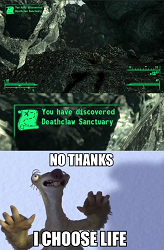
\includegraphics[width=\figwidth]{pics/6/17.png}
	\end{center}
\end{wrapfigure}
This quick burst of violence was followed by a short whispered debate about what to do next. 
We had a few handguns, a couple knives, a handful of detpacks, and a whole bunker full of cultists to deal with. 
This is where your typical Inquisition strike force would have ventured into the temple and purged the entire place using nothing but some silenced handguns and their wits. 
We did not decide to do this, we preferred life. % TYPO prefered -> preferred

The elevator wouldn't budge, but the Adept refused to take the stairs, so we all got into firing positions around Twitch while he fiddled with the control console. We were all on edge, any second the rest of the temple would notice the two missing cultists and come for us. Our nerves were not helped by Crisp pointing out a picture of a man being pierced by what appeared to be an obscene power weapon or the Adept pointing out a few women who looked like Doc's 'ladyfriend'.

The horde of deranged cultists never came though,Twitch bypassed the lock on the elevator relatively quickly and we all piled on. As we rode up we took the few detpacks we had brought and stuck them to the shaft's walls; the general theory was to call in an orbital strike when we got clear, but it wouldn't do to have anyone follow us. We reached the vault doors without any alarms going off and used the built in comm system to nicely ask the guards to let us out.

As we came out of the doors the guards all caught site of the Adept and took a step back, we left the building without incident. As soon as we were clear we commed the diplomatic team and sprinted for the rented rooms where we had stashed our weapons. We grabbed our gear, headed for the parked flier, and got aboard right as Twitch's detpacks went off. 

We could hear small arms fire plinking off the belly of the flier as we lifted into the air and got the hell away from there.

\begin{wrapfigure}{O}{\figwidth}
	\begin{center}
		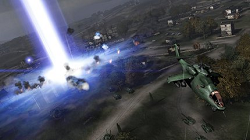
\includegraphics[width=\figwidth]{pics/6/18.png}
	\end{center}
\end{wrapfigure}
The Rupert was a little cross about the whole thing. He'd been working hard at winning the locals over and had expected a report on our progress and a request for a local strike team, not a message to drop everything and evacuate. According to him the local baron and his cronies were "Fine, upstanding gentlemen eager to mend fences with the Imperium and perfectly willing to lend us some lads who could keep their gobs shut". Alfred silently shook his head in the background and did his best to indicate that the 'gentlemen' would have had us all killed, looted, and possibly eaten.

Regardless of how well the Rupert had actually been doing at winning the locals over, setting off a few detpacks in their primary tourist attraction had definitely pissed them off. The Interrogator complained bitterly about all of his diplomatic work being wasted and how hard it would be to get this town back on good terms with the Imperium, our request for an orbital strike on the bunker didn't improve his mood. We got quite the lecture about a soldier's responsibility to face danger and protect civilians; if it weren't for the steady hail of small arms fire that bounced off the belly of our flier as we took off he would have probably ordered us all back down there.

With Alfred's help Sarge managed to finally calm the Rupert down and convince him to call in the strike. 
As we flew back to the surveyor's camp we saw a series of flashes in the distance and a confirmation was voxed in from one of the frigates patrolling the system. %TYPO voxxed -> voxed
It was a shame they we didn't have any plans for the bunker, just an estimate on the depth and direction from the entrance shaft, they wound up burning down twice as far as we estimated and walked their lance battery in a pretty wide area to be sure the bunker was wrecked. 
The barrage also wiped out half the town, the Rupert was a bit sore about that.

\begin{wrapfigure}{O}{\figwidth}
	\begin{center}
		
\includegraphics[width=\figwidth]{pics/6/19.png}
	\end{center}
\end{wrapfigure}
When we landed back at base the Interrogator went off to work on damage control. 
As he left he was muttering to himself about the political impact of calling in lance strikes on the survivors of a planet wide orbital bombardment. 
We felt a little bad about that, but hey, we were still alive and mostly sane. 
We all went to grab some food and sleep, then got together to figure out what the hell to do next.

Cutter didn't do this lame detective stuff and Doc knew when he was out of his depth, they both wanted to call in some help. 
Crisp put forward the rather disturbing plan of lightly bombarding all the mapped settlements and seeing if any fought back with daemons or sorcery. 
He laughed afterwards, so it was probably a joke, probably. 
Twitch thought the entire planet was one massive cult and we needed to call in the Inquisition, when we pointed out that WE were the Inquisition he suggested that we call the "double Inquisition. 
The Inquisition that inquisites the Inquisition." We put that down as another vote for calling in reinforcements. 
Sarge wouldn't have any of that though, he was certain the Rupert wouldn't call for help unless things got absolutely dire, so he wouldn't embarrass the whole team by asking until we had exhausted all available options.

The only major source of clues we could think of has just been turned to a pit of slag and glass, this just left talking to people and searching through records. 
Neither of these were our strong suit, so we just dumped that job on the rest of the team. % TYPO justed -> just
They quickly established that while most of the surveyors didn't know anything useful, the Ecclesiarchy scribes and that one sister dialogus had records on all the local religions. 
While the Adept and the rest poured through the piles of tedious documentation, we did minimal social legwork needed to keep the Rupert happy and tried to stay out of everyone's way. 
Unfortunately bored guardsmen have a way of getting into trouble.

\begin{wrapfigure}{O}{\figwidth}
	\begin{center}
		
\includegraphics[width=\figwidth]{pics/6/20.png}
	\end{center}
\end{wrapfigure}
Twitch kept to himself and did his usual thing while Sarge tried to keep everyone out of trouble and in shape. 
Crisp and Cutter spent their time cooking for the camp and hitting innocent training dummies with a sword respectively. 
Doc spent more and more time using the base's long range secure vox to talk to the Hospitaller while she helped the sisters with whatever they were doing, it was probably a grievous misuse of his inquisitorial authority. 
Then one night he asked us if we wanted to go down and lend the sisters a hand, apparently there was some minor trouble at one of the larger settlements and having some big strong men around would make thing so much better. 
We all snickered at this lame excuse and packed our bags.

It was remarkably easy get the Rupert to let us off the hook, we weren't really doing anything productive at base and "liaising with the Ecclesiarchy" sounded like something we should be doing. 
He sent us off with his blessing on a transport that was taking supplies out to the sisters, we didn't even bother informing the rest of the team, Doc would have died of embarrassment if we had told the Adept. 

We were all ready to do our duty as fellow soldiers and wingmen, we would valiantly throw ourselves on whatever psychotic battle nuns were in the area while Doc went in for the kill. 
A few hours later we were all in full biohazard suits acting as nurses in a feral world plague ward. 
Thanks Doc.

\begin{wrapfigure}{O}{\figwidth}
	\begin{center}
		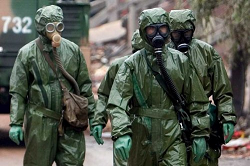
\includegraphics[width=\figwidth]{pics/6/21.png}
	\end{center}
\end{wrapfigure}
In retrospect we really should have looked more closely at the crates we had been sitting on during the flight, every one of them was filled with medical supplies or building materials. 
The moment the transport landed the Hospitaller and a few of her friends started bossing us around. 
They used that medical corpsman tone of voice that every guardsmen is trained to obey, we went from highly trained Inquisition agents to obedient grunts in seconds. 
Before any of us could figure out what was going on we'd built a field hospital, been crammed into biohazard suits, and were being ordered around by a bunch of scary doctor women.

The field hospital was actually pretty large, it wasn't just us and the medical sisters, there were several ecclesiarchy doctors and workers running around too. 
We weren't really expected to help with the medical procedures, thank the Emperor, instead we were moving bodies and equipment around and 'calming down' some of the less happy patients. 
We could see why they wanted a few guardsmen around, some of the locals were very unhappy about their treatment for some reason, we all got a few bruises keeping them still and Twitch nearly lost a finger to a biter.

The day crawled on and we toiled and fought with angry patients while Doc worked shoulder to shoulder with the Hospitaller. 
We all gave him dirty looks every chance we could get, but he didn't seem to notice. 
Eventually there was a lull in the flow of patients and all of us except for Doc stepped out for minute. 
What we saw surprised the hell out of us, the field where discharged patients were being laid was filled with empty spots, the pile of corpses behind the hospital had grown unbelievably large, and the sisters of battle were having trouble holding back a very angry mob.

It occurred to us that there were probably more important things we should be doing than helping Doc get some.

\begin{wrapfigure}{O}{\figwidth}
	\begin{center}
		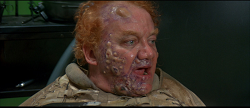
\includegraphics[width=\figwidth]{pics/6/22.png}
	\end{center}
\end{wrapfigure}
We ran back inside, grabbed Doc and the Hospitaller and asked them just what the hell was going on here. 
The Hospitaller explained that during their mission here she had encountered several people showing signs of highly virulent, but curable, diseases. 
She had immediately called in all available personnel to contain the sickness and save as many people as possible. 
The sheer number of locals infected was staggering though, as was the variety of diseases afflicting them, it was amazing that there were any still alive.

Doc claimed to have encountered over fifty different diseases throughout the day, the patient he was currently working on had no less than ten of them, including 'rock lung', 'green death', and 'grox pox' all of which should have been instantly fatal. 
The Hospitaller helpfully pointed out that 'grox pox' was actually a disease that afflicted grox not humans, but confirmed that there was no way the patient should be alive much less sitting up and cheerfully scratching his boils.

While Crisp laughed about the 'grox pox' a heavily blushing Doc administered the drug cocktail that would suppress the patient's numerous diseases, we all watched in horror as the man fell over twitching and screaming. 
Doc muttered something about not being such a baby, called for a stretcher, and moved on to the next patient. 
Sarge pondered the fact the squad's medical officer had not only diagnosed a human with a livestock disease, but also didn't see anything strange about his cure leaving the patient in much worse shape. 
He vaguely wondered if all the interrogators and other inquisitorial agents who had dismissed the squad as a bunch of bumbling idiots didn't have a point.

Sarge's reverie lasted about a second, then he smacked Doc upside the head and bawled him out for not connecting any of this with the fact that there was Nurgle cult somewhere on the planet.

\begin{wrapfigure}{O}{\figwidth}
	\begin{center}
		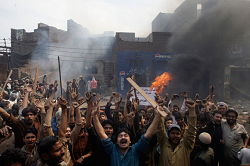
\includegraphics[width=\figwidth]{pics/6/23.png}
	\end{center}
\end{wrapfigure}
The reaming was interrupted by the sound of bolter-fire from outside, we all grabbed our weapons and rushed out to see what was going down. 
Either the mob or the sisters doing crowd control had snapped, the sister superior and her squads were all pouring bolter fire into an onrushing tide of angry locals. 
It should have been over quickly, the first few ranks of angry civvies should have been mowed down and everyone else should have remembered urgent appointments elsewhere. 
They didn't stop coming though, every one of them the sisters shot was simply trampled down as the mob pressed forward baying for blood.

If they had been guardsmen with lasguns things might have gone poorly for the sisters, but a bolter packs a bit more punch and power armor tends to shrug off little things like thrown bricks or small arms fire. 
They held position and mowed down wave after wave of what we were beginning to suspect were nurglite cultists. 
We watched them for a while, purely to make sure they didn't need our help, not because we found a bunch of hot chicks holding the line to be incredibly sexy or anything, then our attention was grabbed by screams coming from the direction of the discharged patients.

Several of the patients were rising to their feet and staggering towards the hospital or the sisters. 
As we watched one of the ecclesiarchy workers tried to get a patient to lie back down, the patient responded by tackling to the ground and tearing at the poor man's biohazard suit with oozing hands. 
We promptly shot the cultist off of him and Sarge loudly ordered everyone who wanted to live to lie down and hold still. 
Something like two of them did, the rest kept coming, so we started shooting them all. 
Doc and the Hospitaller were not very happy about how we were solving the problem.

\begin{wrapfigure}{O}{\figwidth}
	\begin{center}
		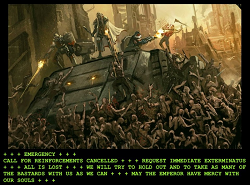
\includegraphics[width=\figwidth]{pics/6/24.png}
	\end{center}
\end{wrapfigure}
The cultists were surprisingly durable, nothing short of a headshot or dismemberment seemed to keep them down, so we took our time and went for kill shots while Cutter and Crisp kept them from getting too close. 
These poor suckers didn't have anything on tyranids or orks, we finished them off without them laying a hand on us, but a few of the ecclesiarchy buys had been caught in the middle of them. 
We got most of them out alive though, except the one Twitch accidentally shot, but no one besides us saw that so it didn't really count. 

Once the internal threat was handled we turned our attention towards securing the perimeter and calling for backup. 
The cultists outside were still trying to get past the sisters, but the fact that their dead completely choked the main entrance kept them to a trickle. 
Twitch brought the sisters some more ammo and went to work on the rest of the perimeter while Cutter and Crisp handled the corpses inside the compound. 
It was sort of disturbing watching them pile up the bodies and roast them in a massive bonfire, especially since Crisp kept cracking up over something.

Doc and the Hospitaller were put in charge the few patients who hadn't tried to kill us. 
Doc seemed a little depressed over the whole thing, which was understandable, as first dates go it really left a lot to be desired. 
Once Sarge was sure everyone was doing something productive he got on the vox and contacted the rest of the team. 
The Rupert was not happy when we asked about the possibility of getting another orbital strike.

\begin{wrapfigure}{O}{\figwidth}
	\begin{center}
		
\includegraphics[width=\figwidth]{pics/6/25.png}
	\end{center}
\end{wrapfigure}
We settled in for the night while the Rupert got the rest of the team together and had a final formal dinner with the surveyors. 
It wasn't that bad really, sure we were sitting in the middle of a miniature zombie apocalypse, but we all had biohazard gear, help was coming, and the perimeter was secured like nobody's business. 
We weren't able to completely slack off though, we had to keep up a rotation with the sisters since the cultists were still periodically rushing the entrance and nurglings were starting the claw their way out of the pile of corpses that choked the entrance.

Despite them being horrific abominations of the warp, we sort of liked the nurglings. 
They weren't very dangerous compared to any of the other daemons out there, they made amusing popping sounds when you killed them, and they were the final proof that this was a chaos cult and not some colossal scew-up on our part. 
We would have sat there killing those disgusting little things all night, but the sisters didn't like them though so we eventually sent Crisp forward to torch the heaps of diseased corpses. 
As the disgusting smoke rolled over us we all thanked the Emperor, and the Hospitaller, for our biohazard gear.

The flames finally convinced the cultists to give it a rest and things stayed relatively quiet until morning when we heard several fliers in the distance. 
The transports landed near the hospital and disgorged several crates of supplies and a bunch of troopers in biohazard gear while a few light fliers scouted the settlement. 
Finally the spiffy flier our team had been using landed near the main entrance. 
The Rupert stepped out, congratulated us on holding the line, and asked for a status report.

\begin{wrapfigure}{O}{\figwidth}
	\begin{center}
		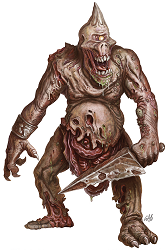
\includegraphics[width=\figwidth]{pics/6/26.png}
	\end{center}
\end{wrapfigure}
We all felt fairly smug as Sarge delivered the report, no one had expected us to find one of the cults on this trip, but we responded quickly and professionally when the cultists showed up. 
The Rupert seemed pretty happy with our report, he happily announced that the only thing that was left to do here was to identify the source of all this disease and purge it. 
We all winced at the thought of walking through a settlement filled with cultists and minor daemons, but orders were orders so we started gearing up for a walk across town.

Luckily we never had to go for that walk, after a few minutes one of the scout fliers reported a large group of cultists heading towards the hospital. 
It wasn't an attack this time, a large shield was carried into the square outside our compound and from behind it a phlegmy voice demanded to talk to our leader. 
Our knee-jerk reaction was to just blow the shit out of them, unfortunately the Rupert was there and ordered us to hold our fire while he walked up to the front of the lines.

With the Greaseball's help our Interrogator actually began talking to the chaos cultists and started trying to negotiate a face to face conversation. 
To the surprise of everyone present he succeeded, an old withered cultist came out from cover followed by a giant of a man with sword and what was unmistakably a plaguebearer daemon. 
We knew how this was going to end, or at least we hoped we did, so while the Rupert started debating with the heretic we got ready for a fight.

\begin{wrapfigure}{O}{\figwidth}
	\begin{center}
		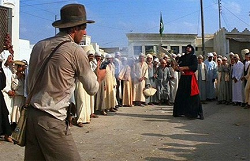
\includegraphics[width=\figwidth]{pics/6/27.png}
	\end{center}
\end{wrapfigure}
The Rupert was holding everyone's attention nicely, no one even noticed as we turned our team's flier around so its side-door was facing the negotiations. 
While Sarge stayed in the flier the rest of us casually cleared everyone out of the way, got Cutter and Alfred in position to grab the Interrogator, and waited for our cue.

Before long the cultist leader had the plaguebearer pull a disease riddled corpse from behind the shield. 
He yelled something about Pontifex's god not protecting him while his faith in Nurgle had made him strong. 
He seemed to think that killing the local religious head was a pretty persuasive argument for conversion. 
The Rupert immediately called the man a vile heretic, drew his power sword, and started to rush forward. 
He didn't get three feet before Cutter and Alfred hit him from the side and dragged his dumb ass out of the line of fire.

As soon as he was clear Sarge slammed open the flier's door and opened up with the side mounted heavy bolter. 
The rest of us supplemented this with frags and las fire while the sisters advanced with their bolters. 
Plaguebearers are supposed to be tough, but it takes more than a little toughness to survive a heavy bolter backed up by grenades, within seconds it was reduced to a greasy stain on the ground along with the cultist leader. 
The big mother with the sword was a different story, he had sprinted forward when the Rupert drew and was dodging and weaving as he closed to melee range.

Cutter revved his chainsword and got ready, then was incredibly disappointed when a bolt round took out the charging cultist's knee. 
We stood around and watched as the maimed swordsman screamed about his tribe killing us all and adding our skulls to the skull throne. 
Crisp asked just which tribe he was talking about, the dumbass told us, then Sarge shot him and we discussed our next steps.

\begin{wrapfigure}{O}{\figwidth}
	\begin{center}
		
\includegraphics[width=\figwidth]{pics/6/28.png}
	\end{center}
\end{wrapfigure}
The Rupert was very understanding about his rough treatment by Alfred and Cutter and was quite happy when we reported location of the khornate cult. 
The large force of cultists the fliers had reported fell back after we killed their leader, but we couldn't just leave them running around. 
We needed to neutralize this cult before we could hunt down the khornates.

We were debating exactly how much purging was necessary when the Adept chimed in. 
She suggested that since we'd removed the cult's leadership and what was probably their only daemon, a full Inquisition team wasn't really necessary. 
She volunteered to stay behind with the sisters and support troopers to oversee the mop up if the Rupert would giver her authority to order limited orbital strikes. 
This seemed perfectly acceptable to all of us, it let us move out immediately and a little old lady didn't really have any place chasing khornate cults. 
The Rupert made a few calls, had a brief meeting with the sisters, then we started loading up our flier for the trip.

As we packed the flier and got out of our incredibly foul biohazard gear we said goodbye to the sisters and the Hospitaller. 
We all snickered as Doc tried to figure out a way to hug her without contaminating himself. 

He didn't and was annoyingly mopey about it for most of the flight.

\begin{wrapfigure}{O}{\figwidth}
	\begin{center}
		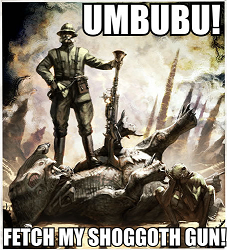
\includegraphics[width=\figwidth]{pics/6/29.png}
	\end{center}
\end{wrapfigure}
Our destination was a jungled area that was known for two things: being home to some of the biggest badasses on the planet and for being absolutely filled with feral orks. 
Twitch was not happy and repeatedly lobbied for simply burning the entire jungle from orbit. 
The Rupert wouldn't have it though, with the exception of the tribe we were heading for the natives here were perfect recruits for the regiments.

We didn't know the exact location of the tribe we needed to purge, the surveyors had just mapped a larger tribal settlement near the edge of the jungle and filled in the rest with 'Here Be Orks', lazy bastards. 
Without a clear idea of where to go, flying around the jungle would be pointless, so we landed near the single mapped settlement and asked around for a guide. 

We had expected terrified muttering and evasiveness from the locals when we asked about the tribe of khornates, but to our surprise everyone seemed to think that they were pretty cool guys. 
Apparently they were just about the best fighters around and would hire out to the other tribes in exchange for food and such. 
We guessed that being near a large concentration of feral orks sort of biases one towards big angry guys that are willing to beat an ork to death with their own severed arm. 
It was pretty easy to get a guide after we explained that we were looking to hire a few of the khornates, and before long we were headed into the jungle behind a young tribal that the Rupert referred to as Umbubu. 
That was not actually his name, the Rupert just called him that.

\begin{wrapfigure}{O}{\figwidth}
	\begin{center}
		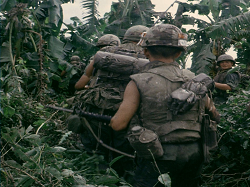
\includegraphics[width=\figwidth]{pics/6/30.png}
	\end{center}
\end{wrapfigure}
If any of us put together a list of things we wanted to be doing 'marching through an ork infested jungle towards a tribe of chaos cultists' would not be high on it. 
In fact it would down at the bottom, right between 'try to ride an angry grox while naked' and 'volunteer to assist a magos biologis with his experiments'. 
We didn't have any choice in the matter though, the Rupert wanted to go so we had to follow. 

We coped with our displeasure in traditional guardsmen fashion, which is to say we complained bitterly about everything and did our best to make sure everyone else was as unhappy as we were. 
This may have been wildly unprofessional behavior, we felt pretty justified though. 
We could have been riding around in our nice comfortable flier, but noooooo, that would 'spook the quarry' and 'draw the wretched greenskins' and 'It was more sporting this way' and 'Umbubu would be too scared to guide us'. 
His name wasn't even Umbubu, it was Chris and that boy grew up next to a jungle full of feral orks, he wouldn't have batted an eye at something as tame as flying after what he'd seen. 
No one listens to a guardsmen, everyone thinks they know better than us.

Really the hike through the jungle wasn't that bad, the Arbite and Umbubu were good at scouting and breaking trail. 
We skirted around the dens of several mutated animals, dodged an ork raiding party, and made sure not to touch any pretty looking flowers. 
Things were just about ideal considering what we were doing, but we still grumbled and Twitch was in a constant state of near panic. 
Twitch did not like orks, or cluttered lines of sight, or loud noises, or sleeping in a position that hadn't been fortified over the last few days. 
To top it off he was dead certain that someone was following us and after a few days the Arbite and Umbubu started agreeing with him.

\begin{wrapfigure}{O}{\figwidth}
	\begin{center}
		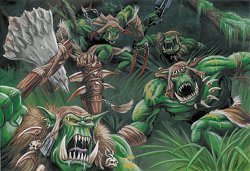
\includegraphics[width=\figwidth]{pics/6/31.png}
	\end{center}
\end{wrapfigure}
Umbubu said we were nearly to the tribe when the orks hit us. 
A twig snapped, a bush rustled and suddenly the Arbite went for his gun and Umbubu was gone. 
Guardsman instinct kicked in and we all dove for cover while Alfred pulled the Rupert and the Cleric behind a tree. 
The barrage of spears missed all of us, except for the Greaseball who now looked a bit like a pincushion, but with more blood and gurgling noises.

The spears were immediately followed by a band of feral orks screaming and waving crude axes as they charged. 
The first few were blown into chunks by the grenades Twitch had tossed on reflex as he grabbed cover and the next batch was taken out by a barrage of las fire, but the last few managed to close to melee range before we could get line of sight. 
Cutter and the Rupert spang into action, power and chain swords whipping across the rushing orks. 
The moment they appeared the entire hunting party focused on them and we took what shots we could get.

The fight was short and surprisingly one sided. 
Cutter was an absolute beast in melee and between his powersword and augmetic arm the Rupert could smash through the orks' crude weapons. 
Both of them fought back to back and any ork that hesitated to get near the whirlwind of death was shot in the back by the rest of us.

After the last ork ran for it and was taken out by a neat shot from the Arbite, Umbubu dropped down from the trees and we gathered together to take stock. 
None of us had been injured, but the Greaseball was dead and both the Arbite and Umbubu were sure more orks would be coming to check out the noise. 
We were getting ready to double time it towards the tribe when a pair of large men with swords stepped out of the jungle.

\begin{wrapfigure}{O}{\figwidth}
	\begin{center}
		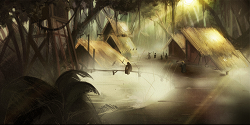
\includegraphics[width=\figwidth]{pics/6/32.png}
	\end{center}
\end{wrapfigure}
Only a quick grab from Sarge kept Twitch from hosing the men with las-fire. 
We all watched with weapons ready as Umbubu greeted the two tribals and introduced us. 
The men were remarkably restrained for khornates, neither seemed inclined to rush us screaming for blood, instead with Umbubu's help they told us to 'come now, children bring your skulls'. 
As we followed them several young tribals came out of the growth and started hacking at the dead orks and the Greaseball's corpse.

None of us felt very comfortable with the situation, but they were taking us where we wanted to go so we rolled with it. 
As we walked the jungle thinned and we started to see headless orks strapped to the trees, as far as border signs went it was pretty effective. 
When we finally reached the village the first thing we all noticed was giant pile of skulls, it was bloody massive. 
At a rough guess there had to be something like five million skulls in that pile, it was amazing that there were any orks left on the planet much less in this jungle. 
We weren't sure how many years they'd been adding to it, but even if it was started the day the planet was nuked it was still damned impressive.

A more educated observer like the Cleric or the Arbite might have made several notes about the tribal's cultural dress and building styles and whatnot, all we noticed was the pile of skulls and that everyone seemed to be seven feet tall and carried a massive sword. 
Our two guides led us a larger hut, instructed us to enter, and left. 
Inside the hut was an old man who looked nothing like a khornate cultist, with Umbubu's help he asked us if we were here to pay tribute, trade, or ascend. 
That last option caught our attention.

We held a quick whispered debate and decided that there probably wasn't any harm in asking what he meant by 'ascending'. 
The old man clarified by asking if we had come from the lesser gods to test our strength and journey to the temple of unity.

Jackpot.

\begin{wrapfigure}{O}{\figwidth}
	\begin{center}
		
\includegraphics[width=\figwidth]{pics/6/33.png}
	\end{center}
\end{wrapfigure}
Really there was no way would say anything but "yes" to that, it was like walking into the armory and being asked if we were there to pick up the new assault bikes. 
Our answer caused a fair bit excitement and runners were sent out in every direction, Umbubu seemed to be about to try and clear up the confusion and explain that we were just looking to hire some mercenaries, but Alfred whacked him around the ear and told him to keep his mouth shut.

What looked like the entire tribe gathered together and formed a ring in the center of the village. 
The old leader asked us who would fight for us to prove our worth, both Cutter and the Rupert immediately stepped forward. 
There was another whispered debate as we tried to convince the Interrogator to leave this to the close quarters combat specialist, but before we could bring him around the leader accepted and ordered both of them to remove their guns and enter the circle.

As they entered several tribals hauled a pair of massive cages into the ring and planet a massive sword in front of each of them. 
The men inside the cages were huge, not just tall and strong like the other tribals, but covered with so much bulky muscle that they looked more like orks than humans. 
Both of them were vibrating with a berserk fury that we could practically feel, we were no longer sure that agreeing to this was a good idea.

Cutter and the Rupert seemed confident though, each man moved in front of a cage, raised their sword, and waited. 
The old leader made a short speech that Umbubu didn't bother translating, the crowd started chanting, the Cleric reached for his flamer and had to be restrained by Doc and Crisp, Sarge had a quick word with Alfred, and with a clang the bolts holding the cages closed were pulled out.

\begin{wrapfigure}{O}{\figwidth}
	\begin{center}
		
\includegraphics[width=\figwidth]{pics/6/34.png}
	\end{center}
\end{wrapfigure}
The two berserkers surged forward, grabbed their swords, and swung at Cutter and the Rupert. 
One could say that it was an epic battle filled with masterful dodges and parries, wounds that left the combatants bloody but even more determined to win, and culminated in a brilliant counterstroke by the underdog. 
One COULD say that, but they'd be lying, it was more like a retarded bullfight.

Cutter dodged the first swing and a follow-up grab, set his chainsword to puree, and just ground it into the berserkers side as he strafed behind the giant. 
The berserker tried to turn and face him, but Cutter was much faster and just kept behind him while the sword dug deeper and deeper. 
We almost felt sorry for the khornate, his muscles were so thick that his arms couldn't even reach behind his back. 
His wildly swinging sword did keep Cutter pinned in close, but you don't need room to swing a chainsword after you get it going. 
It was more like watching someone cutting down an especially screamy tree than a fight.

On the other side of the ring the Rupert had apparently adopted pacifism. 
There was no blood, there were no cunning ripostes, the man just stood there and parried or dodged every attack. 
It was annoying for both the berserker and us in the audience, the man never took an opening, he just stood there. 
The Rupert seemed perfectly willing to drag the fight out until Cutter was finished or the enemy died of exhaustion. 
We could all see the berserker getting more and more frustrated, as the fight wore on he switched to massive charges in an attempt to overwhelm the smaller man. 
Of course the Rupert neatly sidestepped these and to everyone's disgust actually let the berserker get back up after a particularly wild charge.

Just as the audience was getting ready to lynch our dandy Interrogator the berserker seemed to trip over his own feet mid-charge and stumbled face first into the flailing sword of Cutter's opponent.

\begin{wrapfigure}{O}{\figwidth}
	\begin{center}
		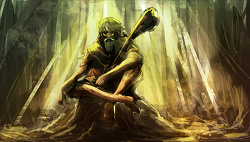
\includegraphics[width=\figwidth]{pics/6/35.png}
	\end{center}
\end{wrapfigure}
The fight ended pretty quickly after that. 
Cutter finished bisecting his enemy and the Interrogator finally gave in to our shouted instructions and decapitated the twitching remains of his berserker. 
He had a sour look on his face, like someone had taken his favorite toy away or insulted his choice of wines. 
As we all walked forwards into the ring we could hear him muttering about it being poor sportsmanship to end a duel so early. 
Sarge quietly thanked Alfred for saving our Interrogator from his own sense of fair play.

When Cutter's berserker had finally stopped thrashing around we all stood before the elder. 
An especially large man with the mark of khorne carved into his chest came and stood before us and a rather surly Umbubu half-assedly translated a speech from the elder. 
It was mostly about the glory of chaos and the big mother's place in our group as the guide to the 'temple of unity' and champion of the blood god, but there was also a bit about leaving immediately and only taking those who would be 'ascending' on the journey.

We paid Umbubu, who was still a little sore at Alfred and the Rupert, and sent the closest thing we had to a translator back home. 
Crisp slipped the kid a few ration-bars and his spare snub pistol, the whole squad had liked the little guy. 
As he left he waved to us and yelled several insults at the Rupert who couldn't understand a word and took as a heartfelt goodbye. 
The we made a note of village's coordinates and followed the big khornate out of the village while all the tribals cheered at us and chanted about blood and skulls.

We felt a little awkward when we called in the village's location and scheduled an orbital strike for later that week. 
The cleric told us that such feelings were caused by the taint of chaos clawing at our minds and prayed for our souls, we ignored him.

\begin{wrapfigure}{O}{\figwidth}
	\begin{center}
		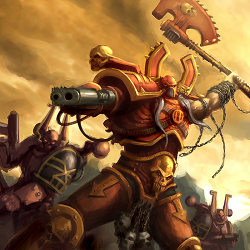
\includegraphics[width=\figwidth]{pics/6/36.png}
	\end{center}
\end{wrapfigure}
We spent a few more days hiking through the jungle behind the khornate towards the 'Temple of Unity'. 
He was actually a pretty nice companion if you ignored the whole 'sworn warrior of the daemonic god of war and bloodshed' thing. 
He would break trail all day long, didn't complain that none of us really spoke his language, and was happy to kill every mutant beast we ran in to. 
He didn't even seem to mind when the Cleric tried to kill him, just watched as we all wrestled the flamer away from the nutcase then went back to eating. 
Crisp really seemed to enjoy talking with him, he had finally found someone who truly appreciated his macabre stories or at least the gesture and tone of them, they'd both stay up late talking and laughing with no idea what the other was saying. 
Hell of a guy that khornate.

We kept in touch with the Adept and the survey base using our long range vox. 
From the sound of it the adept and the sisters were just about done with the nurgle cult, it was just a matter of hunting down the ones who had fled the settlement. 
That vox unit was a bitch to carry, but it was worth it to keep up to date on what was going on and make sure that a record of our discoveries survived. 
We were hoping that once we found the temple we could call in another orbital strike and call it a day, but as we approached it the vox started running into interference and eventually became completely useless. 
We still had to carry the heavy thing though.

The day after the vox unit cut out we reached the 'Temple of Unity'. 
The khornate seemed almost reverential as he entered the clearing and to be fair the temple was pretty damned impressive. 
Damned being the operative word, the place hurt to look at. 
It was mostly stonework that looked ancient as hell, but more recently it had been covered with all sorts of spikes and the eye-watering sigils of each of the four chaos gods. 
It looked like we'd found the final cult.

\begin{wrapfigure}{O}{\figwidth}
	\begin{center}
		
\includegraphics[width=\figwidth]{pics/6/37.png}
	\end{center}
\end{wrapfigure}
While we took in the sight of the chaos temple the khornate planted his sword in the ground and went to his knees in what looked like prayer. 
While the khornate's eyes were closed the Cleric quietly drew his hand cannon, took careful aim, and blew the big guy's head off. 
This caught us all off-guard and Twitch had his gun halfway out before we figured out what had happened. 
The Rupert was rather acerbic and we all expected Crisp to fly into a rage, but the portly flame trooper just laughed and shook his head at the whole situation.

No one was very happy with the Cleric after that. 
Sure it needed to be done eventually, but he had been rather unilateral about it, none of us had even been consulted. 
To make matters worse the edge of the clearing was now covered by a darkly glowing barrier that Alfred told us not to touch, without the khornate we had no way to get out. 
So with no exit and no functioning vox to call reinforcements with our only real option was to just go in and kill everyone. The Cleric heartily approved of this plan and we all told him to shove it.

Our survival gear was stashed in some handy ruins and we all loaded up for a serious fight, there'd be no pussyfooting around with disguises and concealed weapons this time. The heavy flamer and the grenade launcher were brought out, dozens of hand grenades were divvied between us all, and Twitch strapped on his entire supply of explosives. We all prayed to the Emperor that we'd have time to recon the temple and set traps before the fighting started, because if a stray shot hit Twitch now we'd all be blown to very small pieces.

\begin{wrapfigure}{O}{\figwidth}
	\begin{center}
		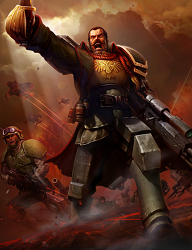
\includegraphics[width=\figwidth]{pics/6/38.png}
	\end{center}
\end{wrapfigure}
The Rupert was in charge of the operation of course, but for once common sense seemed to be triumphing over his love for epic battles and heroic charges. 
As the only remotely sneaky member of our group the Arbite was sent forward to scout the area while the rest of us stayed in cover. 
As he snuck around the temple a basic plan was formulated by the Rupert and delivered along with an inspiring speech about dying for the Emperor. 

Once the main entrance and as many side entrances as possible were located we would all move up to a position with a clear line of site. 
After that Twitch, Crisp, and Cutter would move to each of the side entrances and plant mines while the rest of us provided cover. 
When that was done we'd blow open the front door, heroically charge into the temple, and 'give Johnny Chaos a taste of Imperial Justice'. 
We were a little iffy on that last part, but mining the doors seemed like a good idea so we went with it.

The plan actually held together for a surprisingly long time. 
The Arbite finished his sweep and got into a sniping position on a high set of ruins while we moved forward and Twitch's party split off. 
Mines were planted, remote detpacks were placed, and there was no sign of the enemy as they moved from door to door. 
Twice the main party had to rebase to keep overwatch on Twitch and as we moved to our third position we finally spotted movement.

We could all see someone moving below us, the question here was whether to let him pass by and hope he didn't notice anything or to try and silently take him out. 
While we quietly debated this the Rupert sprang to his feet, yelled 'What Ho foul heretic!' and sent a hail of bolt rounds at the figure.

\begin{wrapfigure}{O}{\figwidth}
	\begin{center}
		
\includegraphics[width=\figwidth]{pics/6/39.png}
	\end{center}
\end{wrapfigure}
The Cleric leapt up next to the Rupert and opened fire as well while Sarge, Doc, and Alfred shared a put-upon look. 
The figure moved with surprising speed towards our position, dodging from cover to cover and drawing a bolt pistol and sword as he ran. 
It was even odds whether he'd make it up to us before our Interrogator or Cleric scored a hit, but luckily the Arbite had a clear shot and a nice leg wound knocked the target down long enough for us to finish the job.

Down on the ground Twitch nearly killed his entire group when the bolt fire surprised him in the middle of mining a doorway. 
He managed to recover though and used his comm to cuss the entire team out until he was interrupted.

Throughout the ruins vox systems blared to life and an incredibly deep voice rumbled out in flawless low gothic. 
It welcomed us to its 'humble temple' and ordered 'all aspirants' to 'deal with the servants of the corpse god and bring any survivors to me'. 
We all heard shouts and chants rising from the various entrances around us, we did not have a good feeling about this.

\begin{wrapfigure}{O}{\figwidth}
	\begin{center}
		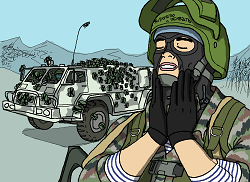
\includegraphics[width=\figwidth]{pics/6/40.png}
	\end{center}
\end{wrapfigure}
So no shit there we were, sitting on top of a chaos temple in the middle of the jungle, surrounded by the sound of daemonically powered warriors baying for our blood. 
We had a nice elevated position and line of site on half the temple, but several of the unmined doors were on the other side of the pyramid we were standing on and Twitch's party was completely exposed. 
There wasn't time to panic, the enemy was coming fast and we had to get ready for a multi-directional attack.

Twitch finished setting his last mines and bolted for a jumble of ruins with Crisp and Cutter on his heels. 
Doc and the Cleric ran around to cover the far side of the pyramid while Sarge settled into position with Alfred and the Rupert. 
The Arbite was ordered to relay enemy positions and only open fire if he saw a hostile we couldn't deal with.

The first aspirant came out a doorway on Doc's side of the pyramid, he and the Cleric immediately opened fire and managed to kill the target before he got ten feet. 
Seconds later we heard the sound of two sets of mines going off and the Arbite reported cautious movement in several other mined doorways. 
Twitch wasn't going to give them time to disarm his mines or fall back, he hit his remote detonator and the entire temple shook as half its exits were sealed. 
We were pretty sure that the explosions or falling rubble killed a bunch of hostiles, but there wasn't time to celebrate since aspirants were pouring out of the remaining side doors as well as the main entrance.

\begin{wrapfigure}{O}{\figwidth}
	\begin{center}
		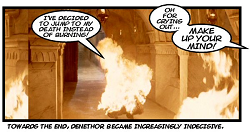
\includegraphics[width=\figwidth]{pics/6/41.png}
	\end{center}
\end{wrapfigure}
What followed was a complete charlie foxtrot. 
These weren't anything like the chaos cultists we'd fought before, each of them was well armed and well disciplined; they were a lot like the traitor guard we had fought back in the regiment, but bigger, stronger, faster, and full of daemonic tricks. 
Some were supernaturally fast and dodged between shots as they dashed towards us while others just ignored their wounds. 
Two of them marched up the side of the pyramid, shrugging off las-fire and hosing Sarge's position with bolter rounds, it took a pair of headshots each from the Arbite to stop them.

Doc and the Cleric were the first ones that were forced out of position. 
Doc was doing a pretty good job of covering the doorways and the Cleric's hand flamer was keeping flankers away, then one of the aspirants started glowing. 
The lightning bolt blew apart their cover and only a quick dive saved Doc from following suit. He and the Cleric fell back towards Sarge's position, as they retreated a pair of aspirants with chainswords came in after them. 
Doc landed several good shots as he ran, but none of them were enough to stop the swordsmen and right as they reached the top of the pyramid the Cleric turned and made his stand.

The closer of the two aspirants was immediately toasted and the Cleric turned towards the second, but a man with a flamer on top of a pyramid is a damned obvious target. 
A round caught the Cleric in the leg and his next burst went wild, only grazing the oncoming swordsman. 
By the time Doc had turned around it was over, the Cleric was dead and three hundred pounds of flaming chaos cultist was charging straight at the wiry medic. 
Doc dodged to the side in the nick of time and the burning aspirant rocketed off the pyramid and started a bone shattering journey down to the bottom. 
A second later Doc overbalanced and followed him a little more slowly.

\begin{wrapfigure}{O}{\figwidth}
	\begin{center}
		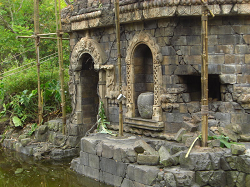
\includegraphics[width=\figwidth]{pics/6/42.png}
	\end{center}
\end{wrapfigure}
Down on the ground Twitch's team was holding their little ruined structure against all comers. 
Cutter and Crisp kept the entrances secured while Twitch took shots at anyone climbing the pyramid and tossed the occasional grenade. 
The enemy made a few attempts to push inside the small structure but each time they were met by a wall of burning promethium or were hit with a chainsword the second they entered the door. 

Between his las-fire and rain of grenades Twitch made it almost impossible for the aspirants to pass his little firebase. 
He was a constant thorn in their side, right up until one of them fielded a grenade and tossed it back.

The grenade almost made it through the window Twitch was crouched under, it was a bit high though. 
The nade went off right where the roof met the wall and with a groan the whole structure started to collapse. 
All three guardsman ran for the exits, but only Crisp made it clear, Cutter and Twitch were both pinned by falling stonework mere feet from the exit.

\begin{wrapfigure}{O}{\figwidth}
	\begin{center}
		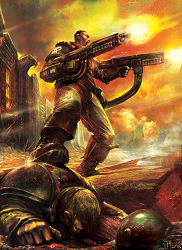
\includegraphics[width=\figwidth]{pics/6/43.png}
	\end{center}
\end{wrapfigure}
Up on the pyramid Sarge was doing the most damage by far with his grenade launcher. 
From his elevated position he could drop rounds on any aspirant who stayed at ground level, only the few who managed to start climbing the pyramid were safe from him. 
Alfred and the Rupert were doing a good job of keeping the enemy pinned for Sarge to finish and between the Arbite and Twitch anyone who managed to get onto the pyramid was quickly sniped off.

Every once in a while Alfred would point out an aspirant that was glowing or had a staff and everyone would redirect fire before something warpy happened. 
Things were looking pretty good, Sarge could see that the enemy was bogged down and running our of reinforcements, then Doc came tumbling down the pyramid and landed at Alfred's feet. 
As the Rupert and Alfred got ready for incoming flankers there was a grinding crash and the ruins Twitch was in collapsed, leaving only Crisp combat-capable on the ground.

Thinking fast Sarge switched targets and rapid fired the last of his grenades at the few remaining hostiles near the collapsed ruins then ordered the Arbite to cover Crisp. 
As he reached for his lasgun the first two aspirants ame around the pyramid were dropped by Alfred and the Rupert, no one was ready for the third.

To his credit Sarge got off a shot before the charging cultist landed on him, it just didn't hit anything.

\begin{wrapfigure}{O}{\figwidth}
	\begin{center}
		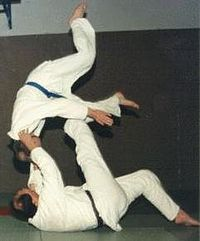
\includegraphics[width=\figwidth]{pics/6/44.png}
	\end{center}
\end{wrapfigure}
A few thoughts flitted across Sarge's mind. 
He wondered why nothing ever worked out as planned. 
He wondered why things kept crushing his chest and if he'd need augmetic ribs after this mission and the previous one. 
Finally he wondered if he should do something about the chainsword swinging towards his head.

Sarge brought his lasgun up just in time to block the chainsword. 
A guardsman's lasgun is a multi-purpose weapon that performs well in several types of combat, this wasn't one of them; the aspirant's blade started ripping through the lasgun with a horrible grinding noise. 
As the whirring teeth neared Sarge's face he summoned every bit of strength he had left, planted his feet in the heretic's stomach and crotch, and heaved.For the second time that day an aspirant tumbled down the pyramid, this one didn't just bounce to the bottom though. 
As the startled heretic flew over the edge and began his descent the last two surviving hostiles that had been pinned on the ground started running up the steps. 

In an ideal galaxy the falling aspirant would have crashed into the other two and all three would have landed in a pile at the bottom of the pyramid, then exploded. 
Unfortunately this isn't an ideal galaxy and only one of them was taken out, but while there was no explosion the activated chainswords both aspirants were holding had about the same effect. 
The surviving heretic continued his charge upwards and reached Sarge's position at the same time as the sorcerer came over the top of the pyramid.

\begin{wrapfigure}{O}{\figwidth}
	\begin{center}
		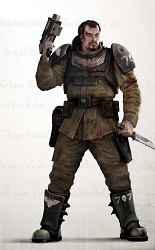
\includegraphics[width=\figwidth]{pics/6/45.png}
	\end{center}
\end{wrapfigure}
It was Alfred who saved everyone, when the sorcerer stepped out and began glowing the butler screamed a warning and put what little power he had into a shield. 
The sorcerer's lightning bolt smashed into the shield and Alfred collapsed to the ground unconscious. 
The Rupert's reaction was perfect, he didn't try to dodge the oncoming bolt, the man had perfect faith in Alfred's shield. 
As calmly as if he were on the firing range the dandy Interrogator took aim and blew the sorcerer's head off. 
Behind him the last aspirant cleared the ledge and took aim with his bolter.

Sarge was down to his holdout pistol and combat knife, but he was ready for this. 
Before the heretic got his shot off Sarge put six inches of good old fashioned Imperial steel into his eye and emptied his stub pistol into the man's gut.

And just like that the fight was over. 

The Arbite commed and told us all hostiles had been eliminated and one by one the squad reported in. 
Doc had a broken arm and a concussion and Alfred was completely out of it. 
Cutter was unharmed, but was trapped in the collapsed ruins and Twitch was buried up to his waist in rubble and might have a broken leg. 
Crisp was relatively unscathed and was trying to dig Twitch out and no one had even shot at the Arbite, the lucky bastard.

While the Rupert held the merely unconscious Alfred and loudly mourned his passing, Sarge appropriated Doc's lasgun and took stock. 
We were down to four combat effective men, the grenade launcher was out of rounds, and there were two wounded and two trapped men that would need looking after. 
The fight was won though and no one important had died. 
All that was left to do was go inside the temple and purge whatever was in it, Sarge eyed the big main temple doors unhappily.

As he watched there was an ominous grinding sound and the doors swung open. 
A giant figure strode out. 

It was nine feet tall and wearing green and blue power armor. 
With spikes on it.

\begin{wrapfigure}{O}{\figwidth}
	\begin{center}
		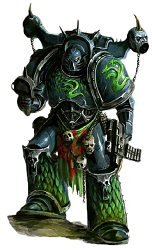
\includegraphics[width=\figwidth]{pics/6/46.png}
	\end{center}
\end{wrapfigure}
Those of us who could still move dropped back into cover and held still, this was not a fight we wanted to have. 
We were wounded, spread out, and only had anti-infantry weapons; we probably couldn't even dent the big bastard's armor much less kill him. 
In our book the ideal weapons for fighting a space marine were a rangefinder, vox unit, and nearby artillery battery and if that wasn't available a Leman Russ might do in a pinch. 
We were not going to try and fight this traitor marine with nothing but lasguns unless we had to.

The marine moved forwards, occasionally kicking a dead aspirant out of the way as he walked to the base of the pyramid. 
Once there he stopped and we all held our breath, then in a booming voice that we all recognized from the vox, he commanded us to stand and face him like men instead of cowering like children. 
We all decided to get in touch with our inner child and did our best to merge with the ground. 

He laughed when none of us responded to his challenge and assured us that he only wanted to talk. 
We had apparently done well to kill all of his aspirants and he was going to offer us a chance to take their place. 
The Arbite chose this moment to shoot him in the back.

Faster than any of us could track the marine spun around, hefted his bolter and fired. 
We all winced as we heard a wet smacking sound and the Arbite's comm cut off, poor dumb bastard.

The marine calmly turned back towards the pyramid and resumed his pitch, which was was honestly starting to sound pretty good. 
He was offering immortality, superhuman strength, a good medical plan, a tremendous upgrade in weaponry, and a chance to not get shot by a traitor marine. 
It would have been a great deal if it weren't for the whole swearing your soul to chaos thing...

\begin{wrapfigure}{O}{\figwidth}
	\begin{center}
		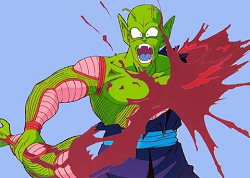
\includegraphics[width=\figwidth]{pics/6/47.png}
	\end{center}
\end{wrapfigure}
The Rupert was getting more and more agitated as the marine talked. 
The man wasn't a complete idiot, but he was proud and didn't have an ounce of pragmatism in him. 
After the third or fourth time the traitor told us the 'Emperor is nothing but a rotting corpse' and recommended that we 'swear allegiance to a real god' something inside our Interrogator snapped. 
For the second time that day he rose out of cover and opened fire while we scrambled to stop him.

The Rupert's shots were well aimed, but the marine was blindingly fast. 
He sidestepped most of the bolter rounds and the only one to hit merely dented a pauldron. 
Once again the marine raised his bolter and returned fire.

Sarge barely managed to catch the Rupert's leg in time. 
He gave it a mighty yank and the Rupert crashed to the ground missing an arm instead of a head. 
It was the remaining flesh arm too, the man curses a blue streak while Sarge tied it off and dragged him back towards Doc. 
Down below the marine laughed and asked if he needed to come up there and lend a hand. 
When Sarge turned him down he laughed some more and asked what we thought of his offer. 
Sarge expressed interest in his pitch and a desire to subscribe to the marine's newsletter, then asked for a few minutes to mull things over.

\begin{wrapfigure}{O}{\figwidth}
	\begin{center}
		
\includegraphics[width=\figwidth]{pics/6/48.png}
	\end{center}
\end{wrapfigure}
Down in the ruins Crisp was watching the the marine and relaying everything to Twitch and Cutter. 
Twitch was wildly brainstorming ways to get his remaining det packs onto the marine and Cutter was complaining that this was all bullshit and someone needed to dig him out. 
Crisp just sat there and quietly laughed at the situation, it was all completely ridiculous. 
He laughed when the Arbite died, then he laughed when the Rupert lost his arm, and he nearly collapsed when Sarge made the crack about the newsletter. 
He removed his combead when Sarge told him to be serious or be quiet.

Eventually the marine ran out of patience, he gave us one last chance to join him before he started killing us. 
Sarge told him to shove it, but Crisp stepped forward.

\begin{wrapfigure}{O}{\figwidth}
	\begin{center}
		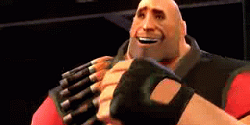
\includegraphics[width=\figwidth]{pics/6/49.png}
	\end{center}
\end{wrapfigure}
The rest of us were floored, both Sarge and Doc scrambled up to get a view as the portly flame trooper holstered his weapon and walked towards the traitor marine. 
We all started shouting, Doc pleaded for his soul, Sarge barked orders and threats in his most commanding voice, Cutter asked what was going on, and Twitch called him 'Traitor McTraitor Pants' and swore that he had known all along. 
Crisp ignored us all, as he walked he laughed and talked to the marine.

He talked about the death he had seen and laughed. 
He talked about the death he had dealt and laughed.

He talked about the faithful men who had died and laughed. 
He talked about his prayers that hadn't been answered and laughed. 
He talked about immortality and the glory of living forever and laughed. 
Finally he talked about madness and laughed like we had never heard before.

The marine laughed too and assured him that in the service of the dark gods madness has purpose. 
He welcomed Crisp as a future brother and asked us all to follow our squadmate's example.

Every one of us screamed at Crisp as he walked towards the marine. When he finally stopped in front of the traitor astartes we all fell silent. 
There was a brief second when there was no sound other than Crisp's laughing, then Twitch hit his detonator.

\begin{wrapfigure}{O}{\figwidth}
	\begin{center}
		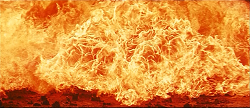
\includegraphics[width=\figwidth]{pics/6/50.png}
	\end{center}
\end{wrapfigure}
Every single one of Twitch's remaining detpacks was stuck to the back of Crisp's flamer tank and the tank itself was at least half full. 
The explosion shook the entire temple and Sarge could feel the heat of the flames from his position near the top of the pyramid. 
There weren't even bodies left, just little fragments of ceramite and a few puddles of burning promethium.

We were all silent and just watched the flames for a few minutes, then the Rupert asked what happened and we all snapped back to reality. 
Doc needed his whole kit to treat the Rupert not to mention his own wounds. 
Twitch and Cutter both needed to be dug out and Sarge was adamant that we find a way to contact someone and tell them just what sort of crazy shit was going on.

Sarge went and grabbed Doc's bags from the stash then went to work with his entrenching tool on the masonry trapping Twitch and Cutter. 
Eventually everyone was collected and stable and it was time to decide what to do.

There really weren't a lot of options, we had to go into the temple. 
Our vox unit still wasn't getting through so we needed to see if there was a better one inside, Doc wanted to see if they had a real medbay, and we definitely couldn't find a way through the glowy wall up here. 
We all just hoped that there was nothing else still running around inside, we were tired of this shit.

All of us formed up behind Twitch and Albert and went through the big front doors.

\begin{wrapfigure}{O}{\figwidth}
	\begin{center}
		\includegraphics[width=\figwidth]{pics/6/51.png}
	\end{center}
\end{wrapfigure}
We had expected there to be blood, corpses, spikes, and daemonic runes everywhere. 
The runes were there, but after the first few dozen feet of stonework the place was surprising clean and ordinary looking. 
It wasn't even dark, there were tasteful little skull shaped lights every few feet, just like in HQ. 
Nothing attacked us as we walked through what we began to think of as 'the facility' instead of 'the temple', apparently everyone who had lived and worked here had died in the battle.

We found various training rooms, sleeping quarters, an armoury full of identical bolters and chainswords, and even a perfectly normal mess hall, we didn't touch any of the food though. 
None of us found anything really interesting until we got to the medbay, when we entered Doc froze and made a sort of high pitched wheezing sound. 
Even the rest of us could see that this place was incredibly well equipped, there were all sorts of shiny machines and tubes and shit. 
After Doc got over the sheer quality of the medbay he commandeered Cutter as a nurse and went to work on his arm as well as the Rupert's bloody stump. 
We left him to it while we checked the nearby rooms.

The next room over gave us a little pause, there were several tanks with what were probably aspirants floating in them hooked up to all sorts of tubes. 
After a short debate we decided that perimeter security trumped preserving evidence and shot them all, but we made sure to hit as little of the fancy machinery as possible, Doc was rather insistent about that. 
The room after that held something that stopped us all in our tracks, Twitch ran back to the Rupert and asked what the Inquisition's standpoint on salvage was. 
He was rather disappointed when he was told he couldn't keep the fully loaded Thunderhawk we found in the vehicle bay, or any of its hellstrike missiles.

The rest of us were similarly disappointed when we realized the Arbite had been the only one who knew how to fly.

\begin{wrapfigure}{O}{\figwidth}
	\begin{center}
		\includegraphics[width=\figwidth]{pics/6/52.png}
	\end{center}
\end{wrapfigure}
Eventually we got to a room with green snake looking thingy on the door. 
This was the first one that was actually locked, but we got in after a little tinkering and finally found where the big vox unit was kept. 
There was a lot of other stuff in there, but aside from a few armor tools and weapons we had no desire to touch none of it was very interesting to us.

It took a while to get the vox system working, but it seemed to punch through the interference no problem. 
We dialed the sisters up and gave a brief rundown of the situation to the Adept, then we went and got the Rupert out of the medbay because she didn't believe us. 

After that it was a lot of talking and waiting. 
Messages were sent to the closest Inquisition base, orders were relayed to the survey base and the ships in orbit, and the remaining sisters were requisitioned to help keep the place secure until a full Inquisitor arrived. 
There was a certain temptation to just blow up the facility, but it wasn't currently doing anything chaosy and someone smarter than us really needed to take a look at this place.

The sisters and the Adept arrived by air, they just flew right over the glowy wall which we STILL couldn't figure out how to deactivate. 
We all set up camp as far away from the temple as possible and covered it with as much holy stuff as the Sisters could bring. 
The Adept said the chaos runes wouldn't have any serious effects, but we didn't want to take any chances.

We kept busy for the next few weeks while we waited for the investigation team. 
Doc spent a lot of time with the Hospitaller who was full of sympathy for his broken arm and helped him with everything. 
Cutter found out how to activate the training remotes in the facility and spent most of the time hitting things with his sword. 
Sarge made Twitch help him clear up the bodies and the fragments of chaos space marine that littered the area and the Rupert went over the whole facility with the Adept.

\begin{wrapfigure}{O}{\figwidth}
	\begin{center}
		\includegraphics[width=\figwidth]{pics/6/53.png}
	\end{center}
\end{wrapfigure}
Eventually the team we requested arrived. 
We were surprised to see not one but three inquisitors step off the shuttle followed by a space marine in black armor. 
The next few days were a blur of interviews which we all found incredibly uncomfortable, especially when the astartes kept asking how we killed the traitor marine. 
That guy made us all very uneasy and Twitch started muttering about chaos marine infiltrators, Sarge hit him and told him to shut up before he got us all purged.

There was a lot of talk which we overheard but didn't pay much attention to. 
There was a bunch of stuff about alphas, and legions, and recruiting worlds, and genes, and seeds, none of it really concerned us. 
We just hung out until they decided they were done with us then got the hell out of there on the first navy ship going back Oak's way.

To our surprise we weren't the only passengers on the ship. 
The entire batch of sisters had apparently seen too much and was being called into Inquisitorial service. 
The Sister Superior and her squads would be joining one of the Inquisitor's retinues, but he had no real need for a Hospitaller and sent her off to be one Oak for reassignment. 
Doc was incredibly happy about this. 

We'd been dreading how mopey he was going to get when it was time to go, but this was almost worse. 
The man was a complete sap and none of us could stand talking to him during the trip home, we couldn't even tease him properly he'd just sort of dreamily nod at anything we said. 
Eventually we just rearranged the cabins so they were next to each other and left them to it. 
At least one of us was getting some.

\begin{wrapfigure}{O}{\figwidth}
	\begin{center}
		\includegraphics[width=\figwidth]{pics/6/54.png}
	\end{center}
\end{wrapfigure}
The trip back went quickly, Sarge spent most of it in the medbay with the Rupert and the Adept getting the report in order for Oak. 
This one was a doozy and it sounded like a story you'd hear in a bar, but the other Inquisitor's reports backed it up so hopefully Oak would believe us. 
We all speculated about whether he'd try to promote Sarge again or if we'd all get an increase in pay or something, not every team can take down a freakin chaos marine.

When we reached Oak's ship Doc bid a tearful goodbye to the Hospitaller as she went off to the damned short bootcamp Oak put all his recruits through. 
The one that was just at the other end of ship. 
It wasn't like she was being sent to the Eye of Terror or something, the little sap. 

After that was done with we all went down to our section of the ship and filled in the rest of the boys about Crisp. 
There were a lot of sad faces at the end of that story, but everyone agreed it was a pretty cool way to go. 
One of the other troopers said the Crisp had signed up with one of the death cults during the last mission, which really did explain a lot. 
We all drank to his memory and hoped he was laughing with the big E.

The call down to Oak's office finally came and we all got to stand there and look decorative while he talked with the Rupert about the mission. 
This time there was no way he could turn down a promotion to full inquisitor, even if he did need another medical leave to go get a second augmetic arm. 
The man glowed with pride as Oak praised him for not only removing the cults that kept the planet from being an excellent recruitment world, but also for finding and destroying a chaos operation that was using it for the same purpose. 
We all winced when he used terms like 'level-headed' and 'keeping your men alive', but overall the man deserved his praise.

\begin{wrapfigure}{O}{\figwidth}
	\begin{center}
		\includegraphics[width=\figwidth]{pics/6/55.png}
	\end{center}
\end{wrapfigure}
When the interview was over and the Rupert finished swearing to come back for us after he got his new arm Oak asked us all to stick around for a few minutes. 
He kept it simple, he was very happy with our performance as a team and wanted to know if there were any requests we'd like to make for our future deployments. 
Twitch was about to say something along the lines 'NO PSYKERS OR CLERICS EVER AGAIN' but Sarge hushed him and pondered the question. 
Finally he asked if the squad as a whole could be issued some more robust weaponry, the lasguns just hadn't been cutting it lately. 
Then as an afterthought he asked if Oak could see to assigning a certain new recruit to permanent shipboard duty instead of sending her out on missions. 
Oak agreed and sent us on our way, Doc was practically skipping as we left

We all headed out for some R\&R. 
We talked with the boys, drank in the bar, and generally had a good time. 
Doc repeatedly made the several hour journey to the training section of the ship and we all gave him shit for it. 
A definite highpoint was receiving a crateful of hot-shot lasguns with a note that said 'Courtesy of Assistant Quartermaster Nubby'.

Eventually our time ran out and we started waiting for our next mission. 
We speculated about what sort of insane interrogator or crazy assignment we'd get this time. 
We had tons of theories but none of them were close to what we actually got.

\begin{wrapfigure}{O}{\figwidth}
	\begin{center}
		\includegraphics[width=\figwidth]{pics/6/56.png}
	\end{center}
\end{wrapfigure}
Instead of a runner telling us to report to a shuttle or a personal visit from our new Interrogator we got orders to report to Oak's office. 
When we entered there was no one else there beside Oak and a single tech-priest.

There wasn't any long mission brief or bullshit about promoting Sarge again, Oak simply said that we had proven to be trustworthy men and he was sending us to assist in the procurement of a new ship for his recruitment fleets. 
We would be acting under his authority and were expected to behave professionally. 
That said he introduced the tech-priest as the agent who would be handling the actual inspection and procurement then sent us on our way. 

We followed the silent tech-priest down to a fancier than usual shuttledand stepped inside. We were met by a bunch of other cogboys who chattered away at the senior tech-priest while we stood there. 
Eventually someone noticed us and a monotone voice directed us towards a side room where we'd meet the 'representative from supply'. %TYPO eventuall< -> Eventually
Sarge opened the door and jumped backwards with a shout.

There are some things that shouldn't be seen from less than a foot away, and Nubby's face was one of them.

